\chapter{Introduction}
\label{sec:intro}
Quick note: The reference list is all the way at the bottom of the document, under a lot of filler content.\\
The figure placement is a bit off, this is because i am writing in latex which automatically places images where they fit best. It requires a lot of tinkering to get them placed correctly and they change position when new text is added. Since i was writing close up to the deadline i did not have time to place them correctly.\\
The reference to the 2019 ipcc report did not work for some reason, could not figure out why. 
\newline
\newline

Meltwater runoff through supraglacial, englacial and subglacial channels is one of the principle processes by which glaciers loose mass. With a ever warming climate, glacial meltwater production is increasing (\cite{IPCC_2019}). Meltwater runoff from the Greenland ice sheet accounts for more than half of the total mass loss to the oceans (\cite{pitcher_smith_2015}). Meltwater runoff contributes directly to sea level rise (\cite{pitcher_smith_2019}). Furthermore, glacial meltwater drainage has a strong influence on glacial dynamics and melting as runoff may both warm the ice and alter basal properties (\cite{pitcher_smith_2019}). There is an ever growing understanding of the importance of the glacial hydrologic system but the topic remains remains sparsely studied (\cite{pitcher_smith_2019}). Due to accelerating mass loss trends (\cite{mass_loss_trend}), new knowledge is needed surrounding glacial meltwater systems, and new technologies have enabled more precise measurements and higher quality dataset collection.
%In recent years interest has picked up around this system due to the accelerating mass loss trends of glaciers, and new technologies are enabling better measurements in the harsh glacial environment.
\section{Aims}
The goal of this thesis was to expand the spatial and temporal range of supraglacial channel measurements and to investigate the potential of machine learning to detect morphological features and to improve geometric reconstructions of glacial channels based on the data collected with a drifter platform. Can machine learning be used to automatically detect channel features like step-risers, knickpoints, meander bends and step-pool sequences? 
\section{Research objective}
In recent years, significant advances have been made in remote satellite sensing for measurements of glacial channels. However, direct measurements of channel properties remain sparse due to the difficult measurement conditions on glaciers (\cite{gleason_2016}). Direct measurements are important as model input to validate results obtained by remote sensing, and to measure subglacial channels, which are inaccessible to remote sensing techniques. Current methods of in situ measurements include dye tracing, doppler current profiling, salt injection, geophysical methods and gas tracing. Emerging technology on a drifter platform has shown great promise for measurements in glacial streams (\cite{pressure_inertia}). 
\newline
\newline
During my field tests I used two different drifter platforms. One submersible multimodal drifter recording the water pressure, as well as three components each of linear acceleration, rotation rate and the magnetic field strength. And one GNSS enabled surface drifter platform. The drifters float passively with the current and require no user input. This allows profiling of long channel segments and of subglacial systems. Drifters are low cost and easily deployed, which makes repeated measurements easy and relatively cheap. The drifter platform has been tested in multiple field tests in 2018, 2019 and 2020  (\cite{pressure_inertia}; \cite{multiscale_change}; \cite{topology_and_pressure}).
\newline
\newline
Subglacial drainage systems are largely unknown due to their inaccessibility for measurments (\cite{pressure_inertia}). However, measurments in supraglacial channels may be useful for investigating subglacial channels. Different features present in supraglacial channels, like meander bends and step-risers, yield charecteristic signals (\cite{multiscale_change}). By classifying these signals we may be able to investigate if the same features are present in the subglacial channels. Machine learning techniques are widely used for classification tasks. When properly applied they can accurately sort large amounts of data. In this thesis i have worked on machine learning algorithms that utilize the drifter data for classification purposes.

\section{Study area}
The measurments used in this thesis were collected from a supraglacial channel on the Kongsvegen glacier. The glacier is located on the west coast of the Norwegian Arctic archipelago of Svalbard [\ref{fig:Study_area}]. Kongsvegen is 26 km long, with a total area of $\sim$100 km (\cite{kongsvegen_study_area}). The glacier terminates into Kongsfjorden with a tidewater front. On the glacier there are slopes ranging from 0.5 - 2.5$^\circ $. Kongsvegen is a surge-type polythermal glacier and is currently in a surge phase (\cite{verge_of_a_surge}). 
\newline
\newline
Kongsvegen was deemed a good site to test the drifter platform for the following reasons: The glacier is sizeable and exhibits a wealth of different channels systems in the ablation period. Aerial imagery confirms the seasonal presence of channels spanning multiple kilometres. Historically, meltwater has been found to drain into large supraglacial channels (\cite{Surge_type_glacier}). Surge events are rare, short lived, poorly understood and thought to be closely related to the subglacial hydrologic system (\cite{burgess_forster_larsen_braun_2012}). To further our understanding of this process it is important to take these measurements while the glacier is actively surging. Finally, there is a parallel project monitoring the glacier lake outburst flood of a Setevatnet, a glacier lake on Kongsvegen. The parallel project created interesting synergies with my project through sharing data and logistics. 
\begin{figure}[h]
    \centering
    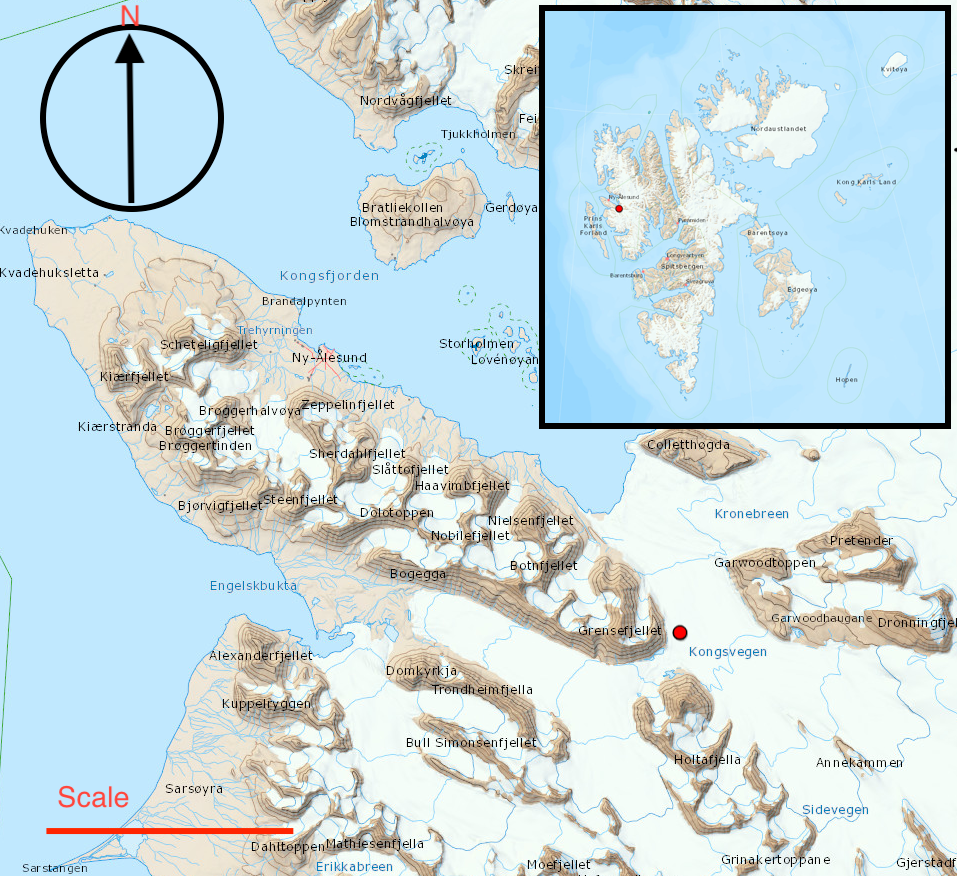
\includegraphics[width = 12cm]{figures/Introduction/study_area.png}
    \caption{Study area on kongsvegen glacier marked by the red dot. This image is a placeholder as i will make a more detailed map in my thesis. The scale line is 10km.}
    \label{fig:Study_area}
\end{figure}

\section{Supraglacial channels}
Supraglacial channels are channels transporting meltwater across the surface of an ice mass. They are found across the entire cyosphere during the summer melt. Channels vary in size from just a few centimetres to tens of meters (Tuhtan et al 2020). The term "channel" is used generically for both streams and rivers (\cite{pitcher_smith_2019}).  Rivers and streams are classified as follows

\begin{itemize}
    \item "Supraglacial rivers are primarily main-stem channels with high stream orders that are perennially occupied. They are regularly spaced, form parallel to ice flow directions, have elongated patterns, and often terminate in moulins." (\cite{pitcher_smith_2019})
    \item "Supraglacial streams are low order with shallow depths, are annual or transient on multiyear timescales, and are often tributary to larger rivers." (\cite{pitcher_smith_2019})
\end{itemize}

Supraglacial channels terminate by draining directly into the sea, onto the terrestrial hydrological system or by entering the subglacial system through moulins or crevasses. Meltwater entering the subglacial drainage system can modulate the subglacial thermal properties, water pressure and dynamic properties like velocity. Alternatively meltwater can remain stored in glacial lakes throughout the winter. If lakes are formed on ice shelves this may cause mass loading and deterioration of ice shelf integrity (\cite{ice_shelf_stability}) (See [\ref{fig:schematic_drain}]).
\begin{figure}[h]
    \centering
    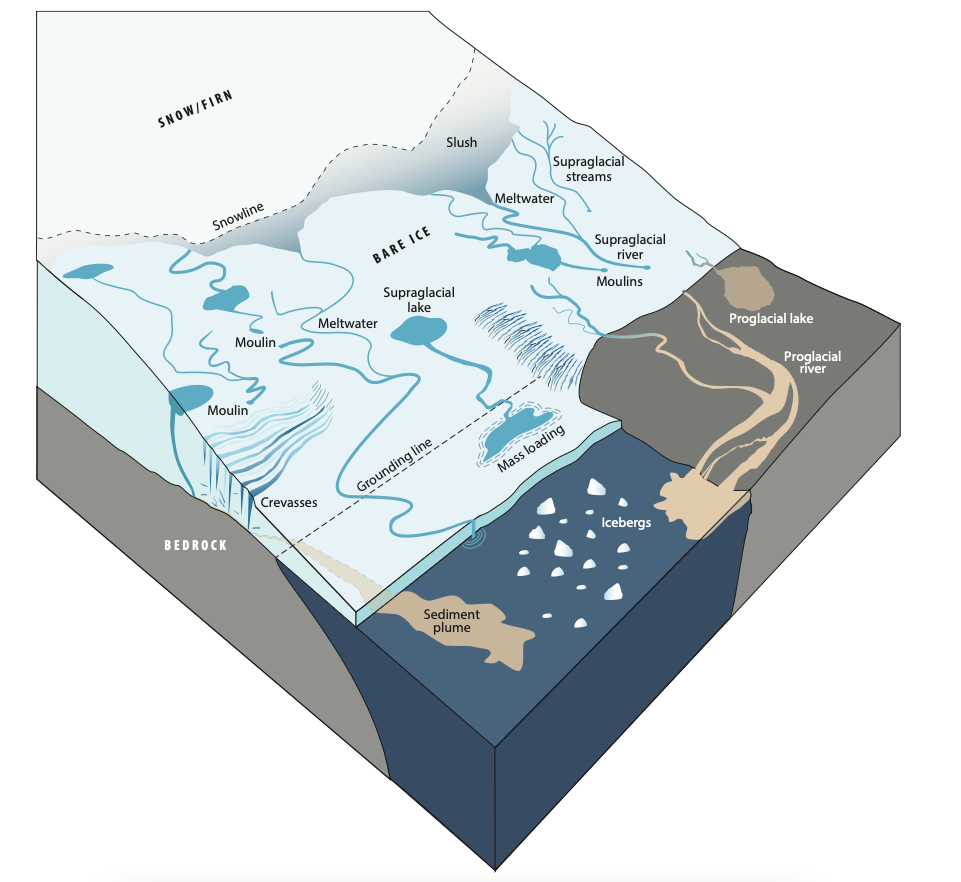
\includegraphics[width = 14cm]{figures/Introduction/schematic_dranage_system.png}
    \caption{ Illustration by Matt Zebrowski, UCLA Department of Geography. Find out if i can use this image}
    \label{fig:schematic_drain}
\end{figure}
\newline
The primary drivers of erosion in supraglacial streams are frictional dissipation of heat from flowing water and thermal erosion from solar radiation. Solar energy input in channels is enhanced as compared to the surrounding ice because of lower albedos. These processes along with other properties like variable melt rates from topographic shading, extensional and compressional ice flow, nonuniform surface slope, variations in ice structure and variations in water input govern channel morphology (Karlstrom et al 2013). 
\newline
\newline
%\textbf{Write something about meandering?}

%\begin{figure}[h]
%    \centering
%    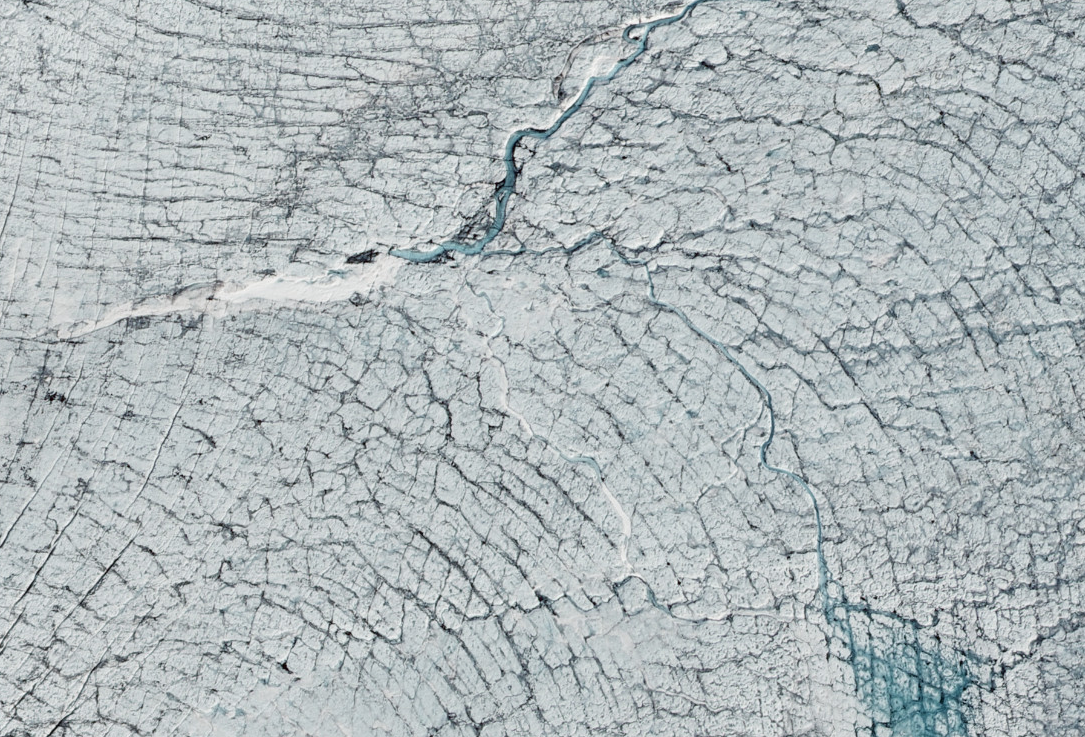
\includegraphics[width = 15cm]{figures/supraglacial_kongsbreen.png}
%    \caption{Supraglacial river on Kongsbreen terminating into a crevasse or moulin. Orthophoto from toposvalbard.}
%    \label{fig:kongsbreen_supraglacial}
%\end{figure}




%\textbf{References to relevant papers:} \\
%Pitcher, L., and Smith, L. (2019). Supraglacial Streams and Rivers. Annual Review Of Earth And Planetary Sciences, 47(1), 421-452. doi: 10.1146/annurev-earth-053018-060212\\\\
%Alexander, A., Kruusmaa, M., Tuhtan, J., Hodson, A., Schuler, T., and Kääb, A. (2020). Pressure and inertia sensing drifters for glacial hydrology flow path measurements. The Cryosphere, 14(3), 1009-1023. doi: 10.5194/tc-14-1009-2020\\\\
%Tuhtan J.A., Alexander, A., Kruusmaa, M., Fuentes-Pérez, J.F. (2020). Multiscale change detection in a supraglacial stream using surface drifters. River Flow 2020, ISBN 978-0-367-62773-7\\\\ 
%Piho, L., Alexander, A., Kruusmaa, M., (2020) Topology and pressure distribution reconstruction of an englacial channel, in review\\\\
%Vatne, G., and Irvine-Fynn, T. (2016). Morphological dynamics of an englacial channel. Hydrology And Earth System Sciences, 20(7), 2947-2964. doi: 10.5194/hess-20-2947-2016


%IPCC, 2019: IPCC Special Report on the Ocean and Cryosphere in a Changing Climate [H.-O. Pörtner, D.C. Roberts, V. Masson-Delmotte, P. Zhai, M. Tignor, E. Poloczanska, K. Mintenbeck, A. Alegría, M. Nicolai, A. Okem, J. Petzold, B. Rama, N.M. Weyer (eds.)]. In press.

%\subsection{Relevant knowns/unknowns}
%\textbf{unknowns:}\\
%There is very little historic data to validate my results.\\\\
%My fieldwork will likely produce huge amounts of data that are difficult to check for quality.\\\\
%Glacial channels can change dramatically over the course of just a few days, this means i am dealing with a constantly changing system and my measurements may yield different results for each of the 45 days i am in the field. This will further complicate the validation process.\\\\
%Many Machine learning algorithms behave like black boxes, you don't know exactly why they are classifying the way they are. This means that they should be used with a lot of care.\\\\
%\textbf{Knowns:}
%Using two different drifter systems that can be collect data independently of each other for validation.\\\\
%Where possible i will use optical imagery as well, perhaps using drones.\\\\
%Previous work has been done on the same platform, but not using machine learning and not on the same scale as my project.\\\\ 
%\section{Aims/objectives}
%Main: Create a method for processing drifter data automatically using machine learning\\
%sub:\\ 
%Detect morphological features\\
%Improve geometric reconstruction of channels\\
%Expand spatial and temporal scale of channel measurements\\
%Improve the drifter platform technology
%\section{Study area}
%Some general remarks about Svalbard and the glaciers there\\
%More about the Kongsvegen glacier where i will be performing my tests.\\\\\\\\



\section{Outline}

The rest of the text is organised as follows:
\begin{description}
    \item[\cref{sec:second}]
    is second to none, with the notable exception of \cref{sec:intro}.
    The main tool introduced here is the employment of unintelligible sentences.

    \item[\cref{sec:third}]
    asserts the basic properties of being the third chapter of a text.
    This section reveals the shocking truth of filler content.

    \item[\cref{sec:fourth}]
    demonstrates how easily one can get to four chapters by simply using
    the \texttt{kantlipsum} package to generate dummy words.

    \item[\cref{sec:first-app}]
    features additional material for the specially interested.

    \item[\cref{sec:second-app}]
    consists of results best relegated to the back of the document,
    ensuring that nobody will ever read it.
\end{description}